%% LLT: Turn off some annoying warnings...
\RequirePackage{silence}
\WarningFilter{titlesec}{Non standard sectioning command}
\WarningFilter{scrreprt}{Usage of package}
\WarningFilter{scrreprt}{Activating an ugly workaround}

% *********************************************************
% CHOOSE THEME (ucph, sund, science, hum, samf, jura, teo)
% *********************************************************
\newcommand{\thesisTheme}{HTLR-Elektronik} % to colortheme and titlepage image


% *********************************************************
% DOCUMENT CLASS
% *********************************************************
\documentclass[%
	paper=A4,					% paper size
	12pt,						% font size
	twoside=true,				% two-sided printing
	openright,					% doublepage cleaning ends up right side
	parskip=full,				% spacing value / method for paragraphs
	chapterprefix=true,			% prefix for chapter marks
	headings=normal,			% size of headings
	bibliography=totoc,			% include bib in toc
	listof=totoc,				% include listof entries in toc
	titlepage=on,				% own page for each title page
	captions=tableabove,		% display table captions above the float env
	draft=false,				% value for draft version
	abstract=on,                % abstract title on/off
]{scrreprt}
\usepackage[utf8]{inputenc}
\usepackage[german]{babel}     % adjust the language

% **************************************************
% COMMANDS FOR REUSE
% **************************************************

% Thesis
\newcommand{\thesisTitle}{Empfangsstation für globales Satellitenbodenstationsnetzwerk SatNOGS}
\newcommand{\thesisSubtitle}{}
\newcommand{\thesisName}{Ritter Gabriel und Metzler Jakob}
\newcommand{\thesisSubject}{Diplomarbeit}
\newcommand{\thesisDate}{2024}
\newcommand{\thesisVersion}{}

% Supervisors & Collaborators
\newcommand{\thesisExternalSupervisor}{}
\newcommand{\thesisInternalSupervisor}{König Christian}
\newcommand{\thesisCollab}{Technische Universität Wien}

% University of Copenhagen
\newcommand{\thesisUniversity}{\protect{Höhere Technische Bundeslehr- und Versuchsanstalt Rankweil}}
\newcommand{\thesisFaculty}{Elektronik und technische Informatik}
\newcommand{\thesisInstitute}{}
\newcommand{\thesisCity}{Rankweil}
\newcommand{\thesisAddress}{Negrellistraße 50}
\newcommand{\thesisPostal}{6830}

% External institution: University of Sussex
\newcommand{\thesisUniSus}{\protect{Technische Universität Wien}}
\newcommand{\thesisUniSusDep}{Space Team}


% *********************************************************
% PACKAGES
% *********************************************************

\usepackage[					% UCPH thesis style
    figuresep=colon,        
    sansserif=false,        
    hangfigurecaption=false,
    hangsection=true,       
    hangsubsection=true,    
    colorize=full,          
    colortheme={\thesisTheme},  % ucph, sund, science, hum, etc.?
    bibsys=biber,
    bibfile=references,       % defines your .bib file
    bibstyle=authoryear,        % refer to https://bit.ly/2YsvIJz
]{ucphthesis}
\hypersetup{					% setup the hyperref-package options
	pdftitle={\thesisTitle},	% 	- title (PDF meta)
	pdfsubject={\thesisSubject},% 	- subject (PDF meta)
	pdfauthor={\thesisName},	% 	- author (PDF meta)
	plainpages=false,			% 	-
	colorlinks=false,			% 	- colorize links
	pdfborder={0 0 0},			% 	-
	breaklinks=true,			% 	- allow line break inside links
	bookmarksnumbered=true,		%
	bookmarksopen=true			%
    }

% *********************************************************
% Cover page content
% *********************************************************
\subject{\vspace{4.5cm} \thesisSubject}
\title{\thesisTitle}
\subtitle{\thesisSubtitle}
\author{\thesisName \\
        \small{Betreuer: {\thesisInternalSupervisor}}
    }
\date{\thesisDate}


% ********************************************************* 
% THESIS CONTENT
% *********************************************************
\begin{document}

% -------------------------- 
% Front matter
% --------------------------
\pagenumbering{roman}
\pagestyle{empty}				            % no header or footers
\AddToShipoutPicture*{\TitleBackground}     % adding background picture
\maketitle                                  % making the title
% Cover back page
\AddToShipoutPicture*{\TitleWatermark}% adding watermark
\hfill
\vfill
{
	\small
	\textbf{\thesisName} \\
	\textit{\thesisTitle} \\
	\thesisSubject, \thesisDate \\
	Betreuer: \thesisInternalSupervisor \\[1.5em]
	\textbf{\thesisUniversity} \\
	\textit{\thesisFaculty} \\
	\thesisAddress \\
	\thesisPostal\ \thesisCity
}

    \clearpage

\pagestyle{plain}
\vspace*{4cm}

\begin{figure}[H]
	
\includegraphics[width=4cm, left]{figures/upper-quote-marks.png}
\end{figure}

\textit{$"$In der Welt der drahtlosen Kommunikation sind Antennen die Stimme, die ohne Worte spricht, aber dennoch eine universelle Sprache vermittelt."} \\
\newline
\rightline{Unbekannt} \\
\vspace{2cm}
\newline
\textit{"Von Anfang an übertraf Maxwells Theorie alle anderen an Eleganz und an der Vielzahl der Beziehungen zwischen den verschiedenen Phänomenen, die sie einschloss."}\\
\newline
\rightline{Heinrich Hertz}
\vspace{1cm}

\begin{figure}[H]
	
\includegraphics[width=4cm, right]{figures/lower-quote-marks.png}
\end{figure}




        % INCLUDE Quotes
\pdfbookmark[0]{Vorwort}{Vorwort}
\chapter*{Vorwort}
\label{chap:Vorwort}
%\vspace*{5cm}
Unsere Diplomarbeit nahm ihren Lauf als einige freundliche Mitglieder des TU-Wien-Space-Teams auf unsere Schule zu kamen und uns ein Projekt vorstellten: eine Bodenstation zum Empfang von Daten eines Satelliten der 2024 in den LEO befördert werden sollte - des STS1.\\
\newline
Dies weckte unser Interesse, bald fanden wir uns in einem Team wieder das hochmotiviert und bereit war loszulegen. 
       % INCLUDE Preface
\pdfbookmark[0]{Abstract}{Abstract}
\section*{Abstract}
\label{chap:abstr}
Shortly before his death, Stephen Hawking advised humanity: \glqq Look up at the stars, not down at your feet!\grqq{} This underscores the importance of space exploration. In order to enable investigations in space, specifically in the Low-Earth Orbit, for students at general and vocational higher schools, the TU Wien Space Team launches a satellite in 2024 as a research platform for this purpose into Earth's orbit. To communicate with this satellite, a global network of receiving stations is required, for which a receiving station is developed, constructed, and put into operation as a case study in this thesis.

\subsection*{A Objectives}
The main objective of this thesis is to successfully receive data from existing satellites in the 70cm band. For this purpose, the receiving station, which is put into operation as part of the work, will be integrated into the global satellite ground station network SatNOGS. This will provide satellite operators with extended geographical coverage for communication and improved reliability.

\subsection*{B Implementation}
As main components of the receiving station an antenna array consisting of four directional monofilament helical antennas and a quasi-omnidirectional quadrifilar helical antenna are developed and constructed. For the necessary tracking of the directional antennas, a Yaesu G-5500DC rotor is used, and the required computer control interface is emulated. All remaining components for the receiving station are compactly housed in a switch cabinet.

\subsection*{C Results}
The result of the thesis is a functional receiving station that receives data from scientific satellites in the 70cm band using both developed antenna types. Additionally, the documentation of the time and financial expenditure allows for the evaluation of the profitability of the respective antenna types and the identification of further advantages and disadvantages.      % INCLUDE Abstract
    \clearpage


\setcounter{tocdepth}{2}		% define depth of toc
\tableofcontents				% display table of contents
    \clearpage


% -------------------------- 
% Main matter
% --------------------------
\pagenumbering{arabic}			% arabic page numbering
\setcounter{page}{1}			% set page counter
\pagestyle{maincontentstyle} 	% fancy header and footer

\chapter{Rationale}
\label{chap:rationale}
Wieso ist das thema relevant, motivation für diese DA    % INCLUDE Rationale
\chapter{Einführung}

\label{chap:Einführung}
In diesem Kapitel werden die theoretischen Grundlagen der Antennen-und Leitertheorie gelegt sowie das SatNOGS Netzwerk näher erläutert.

\section{SatNOGS-Netzwerk}
\label{sec:sat}
Das SatNOGS-Netzwerk spielt eine zentrale Rolle in unserer Diplomarbeit und bietet hunderten Forschern, Amateurfunkern und Interessierten eine Plattform für verlässliche Kommunikation mit Satelliten.\\

Das, was SatNOGS zu so einer attraktiven Lösung macht, ist der Fakt dass die Bodenstation um den ganzen Globus verteilt sind. Der große Vorteil davon ist, dass der Empfang von Satellitendaten nun über alle verfügbaren Empfangsstationen laufen kann.\\

In Abbildung \ref{fig:SatNOGS_Erklärung} wird die Topologie des SatNOGS-Netzwerkes abstrahiert dargestellt.
Alle über das Netzwerk verfügbaren Bodenstationen sind mit SatNOGS-Servern verbunden. Auf diese Server kann über die Website bzw. API zugegriffen werden, welche die empfangenen Satellitendaten für alle Benutzer erreichbar macht.

\begin{figure}[H]
	\centering
	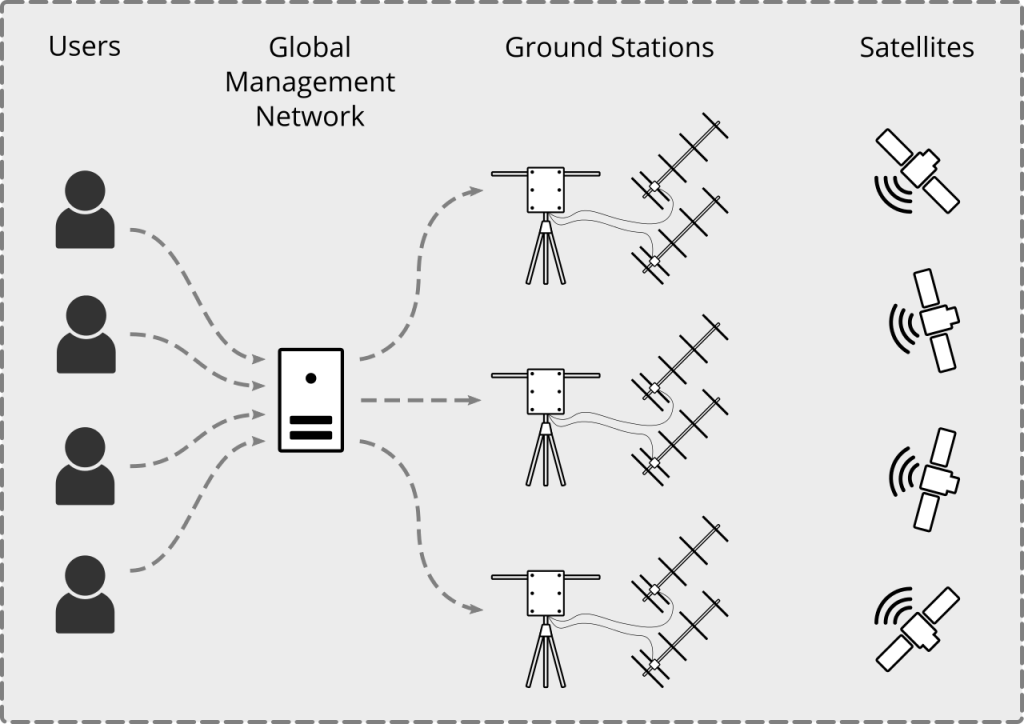
\includegraphics[width=\textwidth]{../ref/SatNOGS_explanation}
	\caption{Erklärung des SatNOGS Netzwerkes}
	\label{fig:SatNOGS_Erklärung}
\end{figure}	

\begin{figure}[H]
	\centering
	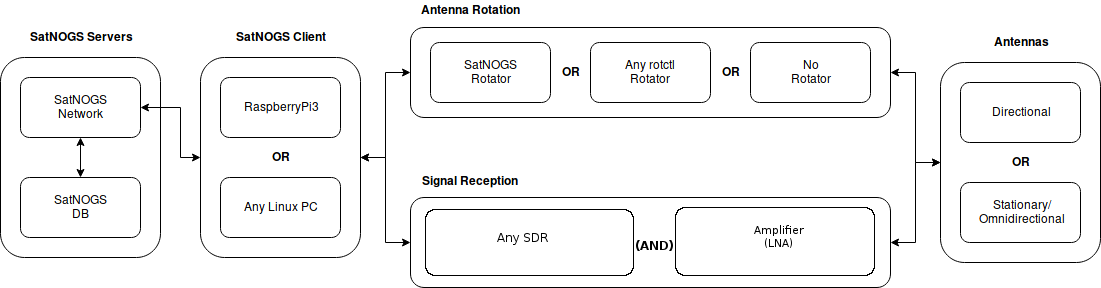
\includegraphics[width=\textwidth]{../ref/SatNOGS_BlockDiagram}
	\caption{SatNOGS-Systemtopologie}
	\label{fig:SatNOGS_Systemtopologie}
\end{figure}

Um näher auf den Ablauf des Datenempfangs und der benötigten Systemblöcke einzugehen wird auf Abbildung \ref{fig:SatNOGS_Systemtopologie} verwiesen.\\

Zum Empfang von Daten kommen zwei Antennentypen infrage: Direktionale oder omnidirektionale Antennen. Eine direktionale Antenne folgt dem Verlauf des Satelliten. Dies bringt den Vorteil mit sich, dass eine höhere Empfangsleistung erzielt, und somit klarere Daten empfangen werden, jedoch wird für solch ein Modell ein Rotator benötigt. Der Vorteil einer omnidirektionalen Antenne ist, dass kein teurer Rotator notwendig ist, allerdings können damit nur schwer brauchbare Daten empfangen werden.\\

Für gerichtete Antennen können verschiedene Rotatoren benutzt werden, unter anderem der "SatNOGS-Rotator" sowie diverse Open-Source-Rotatoren und Rotatoren welche zum Verkauf stehen.\\

Zur Demodulation der Daten sind ein SDR (Software Defined Radio) sowie ein LNA (Low Noise Amplifier) notwendig. Das SDR übernimmt softwaretechnisch Aufgaben welche normalerweise von Hardware übernommen werden (Demodulation, Filter, Mixer, etc...). Der LNA, wie der Name schon andeutet, ist für die Verstärkung kleiner Signale mit besonderer Rauscharmut verantwortlich. \\

Die Aufgabe des SatNOGS Clients kann in der Regel von jedem Linux-PC oder RaspberryPi übernommen werden. Allerdings wird die Kompatibilität zwar für alle Linux-basierten PCs, jedoch nur für die RaspBerryPis Version 3, 3+ und 4 garantiert.\\

Der SatNOGS Client ist mit den Servern verbunden, der die Bodentation als solche im Netzwerk repräsentiert. Die Server unterhalten weiters eine Datenbank, welche Daten über Satelliten enthält, die mit den Empfangsstationen erreichbar sind.
\pagebreak
\section{grundlegende Antennentheorie}
\label{sec:basic-ant}
\subsection{Einführung}
Um die in der Diplomarbeit bearbeiteten Inhalte besser verstehen zu können, wird eine Einführung in die Grundlagen der Antennentheorie gegeben. 

\subsection{Antennenfeldzonen}
Das von einer Antenne abgestrahlte Feld lässt sich in 3 verschiedene Regionen einteilen: das Nahfeld, das Übergangsfeld (Fresnel-Region) und das Fernfeld (Fraunhofer-Region).\\
\newline
Je nach Literatur erfolgt der Übergang zwischen den Feldzonen fließend. Eine Möglichkeit die Zonen einzuteilen ist in der nachfolgenden Tabelle einzusehen.

\begin{center}
	\begin{tabular}[h]{|c|c|c| p{"5"cm}}
		\hline
		Nahfeld & Übergangsfeld & Fernfeld\\
		\hline
		r $<$ 0.2 $\lambda$ & 0.2 $\leq$ r $\leq$ 4$\lambda$ & r $>$ 0.4$\lambda$\\
		\hline
	\end{tabular}
\end{center}

Das Nahfeld ist darin besonders, dass das elektrische und magnetische Feld mit unterschiedlichen Faktoren in Abhängigkeit der Entfernung abnehmen. Im Übergangsfeld nehmen das elektrische und magnetische Feld zwar mit dem gleichen Faktor ab, jedoch unterscheiden Sie sich noch in der Phase und Amplitude.\\
\newline
Im Gegensatz zum reaktiven Nahfeld wird beim Fernfeld Wirkleistung abgestrahlt. Hierbei sind die elektrische und magnetische Komponente der Welle in Phase und nehmen im gleichen Maß ab.\\
\newline
Da unsere Diplomarbeit einen Fokus auf die Satellitentechnik hat, ist für dieses Dokument nur das Fernfeld relevant. 

\subsection{Polarisation}
Die Polarisationsart wird von der Ausrichtung des Vektors der elektrischen Feldstärke bestimmt. Es lässt sich zwischen drei verschiedenen Arten der Polarisation unterscheiden.\\
\newline

\begin{itemize}
	\item Lineare Polarisation
	\begin{itemize}
		\item horizontale Polarisation\\
		Eine horizontale Polarisation liegt vor, wenn der elektrische Feldstärkevektor sich periodisch ändert und die Feldlinien parallel zum Boden verlaufen.
		\item vertikale Polarisation\\
		Eine vertikale Polarisation liegt vor, wenn die elektrischen Feldlinien senkrecht zum Erdboden liegen.
		Eine vertikale Polarisation liegt vor wenn
	\end{itemize}
	\item Zirkulare Polarisation\\
	Der Betrag des elektrischen Feldstärkevektors ist konstant. Der Feldstärkevektor rotiert in einer Spirale um den in Ausbreitungsrichtung weisenden Vektor. Ein Spiralumlauf ist nach der Wellenlänge $\lambda$ vollendet.
	\item Elliptische Polarisation\\
	Betrag sowie Richtung des elektrischen Feldstärkevektors ändern sich laufend. Bei der Rotation beschreibt der Vektor eine Ellipse.
\end{itemize}
linear (vertikal, horizontal), Zirkular, Elliptisch

\subsection{Kenngrößen einer Antenne}
abc

\subsection{Antennengewinn}
Als Antennengewinn wird die $"$bündelnde$"$ Eigenschaft einer gerichteten Antenne im Vergleich zu einer Bezugsantenne bezeichnet. Hierbei ist die Vergleichsantenne meist ein Kugelstrahler.\\
\newline
Der Gewinn der Antenne berechnet sich mit dem Verhältnis der maximalen Empfangsleistung der gerichteten Antenne zu der des Kugelstrahlers. Wird als Bezugsantenne der Kugelstrahler verwendet, so wird die Empfangsleistung mit dem Index 'i' versehen um dies zu kennzeichnen.

\begin{equation}
	G=\frac{P_{max}}{P_{i}}
\end{equation}

\paragraph{Welligkeit}
Die Welligkeit oder das Stehwellenverhältnis (SWR) gibt Aufschluss über die Spannungsverteilung auf der Speiseleitung und ist ein Maß für die Qualität der Anpassung. Sie beschreibt, wie groß der Anteil der reflektierten Wellen ist. Je schlechter die Anpassung, desto größer der Anteil der Wellen, welche reflektiert werden.\\
\newline
\begin{equation}
	SWR=\frac{U_{max}}{U_{min}}=\frac{I_{max}}{I_{min}}=\frac{1+\lvert \rho \lvert}{1-\lvert \rho \lvert}
\end{equation}

Wobei $\rho$ der Reflexionsfaktor ist. 

\paragraph{Richtcharakteristik und Richtdiagramm}
Die Richtcharakteristik beschreibt das Abstrahlverhalten einer Antenne. Hierbei wird die unter einem bestimmten Winkel ($\theta$, $\phi$) auftretende Feldstärke auf einen Maximalwert bezogen.

\begin{equation}
	C(\theta, \phi)=\frac{E(\theta, \phi)}{E_{max}}
\end{equation}

Wobei $\theta$ der Elevationswinkel (vertikal Winkel) und $\phi$ den Azimutwinkel (horizontaler Winkel) repräsentiert.

\begin{figure}[H]
	\centering
	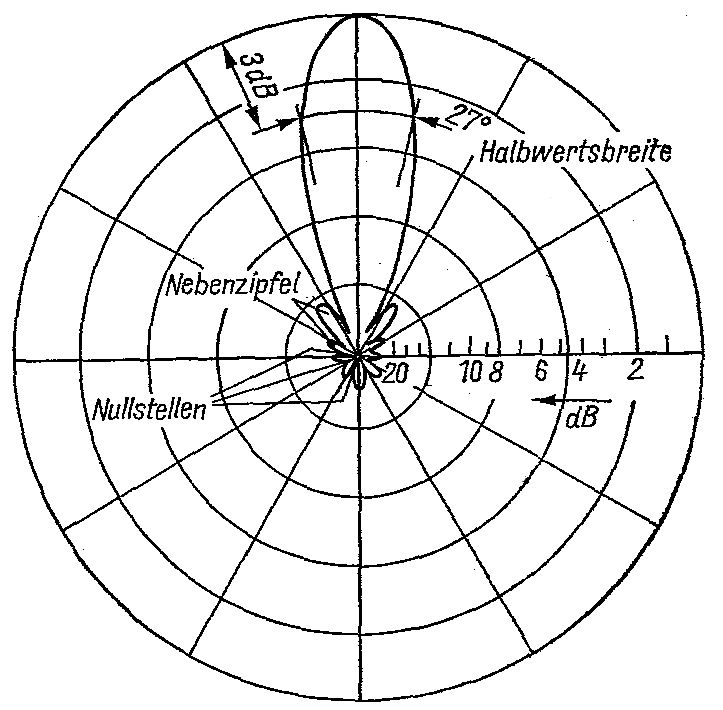
\includegraphics[width=\textwidth]{../ref/Richtdiagramm_Beispiel}
	\caption{Richtdiagramm einer stark bündelnden Antenne}
	\label{fig:Richtdiagramm Beispiel}
\end{figure}

Hierbei ist zu bemerken dass in Abbildung \ref{fig:Richtdiagramm Beispiel} entgegen der üblichen Konvention das Richtdiagramm aus dem Verhältnis zwischen Strahlungsleistungsdichte und ihrem Maximalwert ergibt. Es ist gebräuchlich, das Diagramm auf den Maximalwert zu normieren, sodass sich bei der maximalen Feldstärke 0 dB Dämpfung ergeben.\\
\newline
Der größte Teil der Leistung ist naheliegend in der Hauptkeule zu finden, während es nötig ist die Neben-und Rückwärtskeulen möglichst klein zu halten, um unnötige Abstrahlung in die Umgebung zu vermeiden. Die Halbwertsbreite der Hauptkeule ist der Wert ab dem die Leistungsdichte auf die Hälfte abgesunken ist.\\
\newline
Eine weitere wichtige Kenngröße bei Richtantennen ist das Vor-Rückwärtsverhältnis. Dies ist die Fähigkeit einer Richtantenne, Strahlung aus anderen Richtungen als der Hauptstrahlrichtung zu unterdrücken.

\paragraph{Einfluss der Erde auf das Richtdiagramm}
Wird das Strahlungsdiagramm einer Antenne über dem Boden mit dem einer Antenne im Freiraum verglichen, lassen sich große Unterschiede erkennen. Der Boden dient als Reflektor wobei seine Reflexionseigenschaften von der Dielektrizitätskonstante sowie der Leitfähigkeit bestimmt werden.\\
\newline
Für die Reflexion elektromagnetischer Wellen am Erdboden trifft das Reflexionsgesetz zu, das bedeutet, dass der Einfallswinkel gleich dem Ausfallswinkel ist. Hierbei kann es zu Überlagerungen zwischen den reflektierten und nicht reflektierten Wellen kommen und somit können destruktive und konstruktive Interferenzen entstehen.\\
\newline
Die Polarisierung der verwendeten Antenne spielt eine entscheidende Rolle bei der Reflexion. Bei einer vertikal polarisierten Antenne ist der Stromverlauf von Spiegelbild und Original gleichphasig. Bei einer horizontal polarisierten Antenne hingegen ist der Stromverlauf zwischen Reflexion und Original gegenphasig.\\
\newline
Der Abstand vom Boden spielt ebenfalls eine kritische Rolle und hat großen Einfluss auf das resultierende Richtdiagramm der Antenne. Wird beispielsweise ein Dipol $\frac{\lambda}{2}$ vom Boden entfernt aufgestellt, so verändert sich sein Richtdiagramm so sehr, dass aus der omnidirektionalen Antenne ein Strahler mit zwei Strahlungskeulen wird. 


\subsubsection{Baluns}

\paragraph{Strombalun}
Mantelwellensperre, schwach gegen statische Entladungen, da Balun -> konvertiert balanced zu unbalanced 

\paragraph{Spannungsbalun}
Konvertiert "balanced" zu "unbalanced" guter Schutz gegen statische Entladung, keine Mantelwellensperre.


\section{QHA (Quadrifilare Helixantenne)}
Die QHA ist eine symmetrische Antenne, was bedeutet, dass sie mithilfe eines Baluns auf ein unsymmetrisches Koaxialkabel angepasst werden muss. Mehr dazu in der Subsektion \ref{subsec:baluns}.\\

Die QHA besteht aus einer größeren Schleife, welche unterhalb der gewollten Frequenz resonant ist, und einer kleineren Schleife, welche oberhalb der gewollten Frequenz resonant ist. Die größere Schleife bildet die kapazitive Komponente und die kleinere Schleife die induktive Komponente. Dadurch entsteht eine Phasenverschiebung von (ideal) 90° über die bifilaren Elemente. Werden die Streifen richtig dimensioniert, so ergibt sich eine gute zirkulare Polarisation, weichen sie ab so ergibt sich eine elliptische Polarisation.\\

Das, was die QHA für die Satellitenkommunikation so attraktiv macht, ist zum einen ihre zirkulare Polarisation, und zum anderen ihre kompakte Bauweise. Diese macht sie einfach transportierbar. Zudem hat sie omnidirektionale Abstrahlcharakteristiken, was den Einsatz eines Rotors nichtig macht. Da die QHA entlang des Horizonts ihren größten Antennengewinn aufweist, macht sie das zu einer guten Wahl für die Weltraumkommunikation\cite{qfh_w3kh_nodate}.

\section{Monofilare Helixantenne}
Die Helixantenne ist die in der Satellitenkommunikationstechnik die am Weitesten verbreitete Antennenart \cite{HelicalAntennas}. Der Grund hierfür ist die Immunität der zirkularen Polarisation gegenüber Faraday Rotation. Dieses Phänomen findet in der Ionosphäre statt MISSING REFERENCE und wurde in (REFERENZ) bereits näher erklärt.

Die Helixantenne hat weiters verschiedene Operationsmodi. Arbeitet die Antenne im Normal-Modus, so zeigt sie ein omnidirektionales Abstrahlverhalten, wobei sie senkrecht zur Achse der Antenne gleichmäßig in alle Richtungen strahlt. Dieser Betriebsmodus wird erreicht, sobald der Umfang einer Windung der Helix im Vergleich zu der Wellenlänge $\lambda=\frac{c}{f}$ klein ist. Der zweite Modus der Wendelantenne ist der Axial-Modus. Befindet sich die Antenne in diesem Betriebsverhalten, so verändert sich die Richtung der Strahlung. Der Großteil der elektromagnetischen Strahlung wird nun entlang der Achse der Spirale abgegeben. Dieser Modus wird erreicht, sobald die Wellenlänge ungefähr gleich groß ist wie der Umfang einer Windung der Spirale \cite{HelicalAntennas}.

Da die Wendelantenne über eine besonders große Bandbreite verfügt, eignet sie sich gut für den Nachbau. Hierbei sind der Durchmesser sowie die Steigung der Spirale von ausschlaggebender Relevanz für die gewünschte Einsatzfrequenz. Der Durchmesser für eine Wendelantenne im Axial-Modus ist hierbei mit $D=\frac{\lambda}{\pi}$ definiert.

Ein Richtwert für die Steigung der Helix ergibt sich empirisch mit einem Steigungswinkel zwischen 12° und 14° \cite{helixWebsite}. Die Steigung der Spirale ist so wichtig für die Funktionalität der Antenne, da sie sich mit einem größeren Winkel eher wie ein Dipol verhält, und mit einem kleineren Winkel eher wie eine Ringantenne. REFERENZ

Die folgenden Bezeichnungen werden zur Beschreibung der Helix verwendet.
\begin{itemize}
	\item D: Durchmesser der Helix
	\item S: Abstand zwischen den einzelnen Windungen
	\item U: Umfang der Helix
	\item $\alpha$: Steigung der Helix
	\item L: Länge einer Windung
	\item n: Anzahl der Windungen
	\item Lges: Gesamtlänge der Helix
	\item d: Durchmesser des Leiters
\end{itemize}

Um den Winkel zu berechnen, lässt sich die aufgerollte Windung der Helix betrachten (Abbildung \ref{fig:Wndg_aufgerollt}).

\begin{figure}[H]
	\centering
	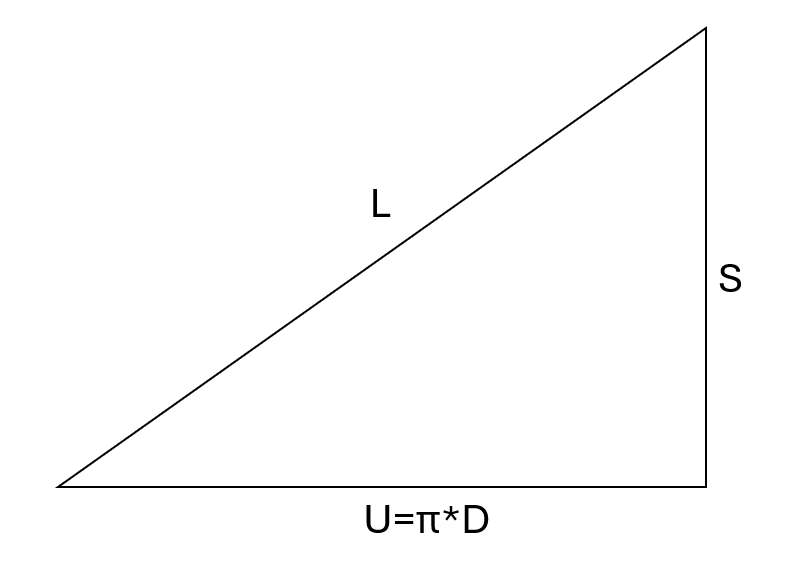
\includegraphics[width=6cm]{../ref/Windung_aufgerollt.png}
	\label{fig:Wndg_aufgerollt}
\end{figure}

Hier lässt sich ein rechtwinkliges Dreieck erkennen. Die Ankathete ist hierbei der Umfang einer Windung und die Gegenkathete stellt den Abstand zwischen den einzelnen Drehungen dar. Somit lässt sich der Winkel $\alpha$ mit der Formel

\begin{equation}
	\alpha=\arctan(\frac{S}{C})
\end{equation}

beschreiben. Ein weiterer vitaler Parameter für die Funktionalität der Antenne ist der Abstand zwischen den einzelnen Windungen. Dieser wird generell für $0,23\lambda$ als ideal angegeben. MISSING REFERENCE

Der Reflektor dient zur Verbesserung der Richtcharakteristik und kann verschiedene Formen annehmen. Er kann kreisförmig, viereckig oder auch trichterförmig sein. Für die Zwecke dieser Diplomarbeit wurde ein kreisförmiger Reflektor gewählt. Als passend wird hierbei ein Durchmesser zwischen $\frac{3\lambda}{4}$ und $\frac{4\lambda}{3}$ angesehen. Der Durchmesser des Leiters ist unkritisch für die Funktion der Antenne, allerdings wird als Richtwert ein Querschnitt von $0,005\lambda$ bis $0,05\lambda$ als passend betrachtet\cite{Kraus-2002-AntennasB}. 

Nachfolgend sind die wichtigsten Gleichungen für die Berechnung der Parameter einer Helix-Antenne gegeben \cite{Kraus-2002-AntennasB}.

\begin{table}[H]
	\begin{tabular}{|l|l|}

		\textbf{Bezeichnung} & \textbf{Formel}\\ 
		benötigte Kabellänge & $L=n*\sqrt{\lambda^2+S^2}$ \\
		D				     & $D=\frac{\lambda}{\pi}$\\ 
		Halbwertsbreite		 & $HPBW=\frac{52}{C*\sqrt{nS}}$ \\ 
		Gewinn               & $G=12*C^2nS$                 \\ 
		Eingangsimpedanz     & $Z=\frac{150}{\sqrt{C}}$      \\ 
		Effektive Antennenfläche    & $Ae=\frac{D*\lambda^2}{4*\pi}$ \\ 
		\end{tabular}
	\end{table}

Anhand der Formel für den Antennengewinn lässt sich erkennen, dass dieser direkt proportional zur Anzahl an Windungen ist. Die Antennenwirkfläche beschreibt, welche Leistung dem elektromagnetischen Feld bei bekannter Leistungsdichte entnommen wird, wie bereits in QUERVERWEIS erwähnt MISSING REFERENCE.

 % INCLUDE Introduction
\chapter{Einrichten des SatNOGS Client}
\label{chap:gs-setup}
Der SatNOGS Client bildet das Herzstück der gesamten Empfangsstation, ist für die Ausführung und Koordinierung der, mit der Empfangstation geplanten, Observationen zuständig und bildet die Schnittstelle zur SatNOGS Datenbank. Das SatNOGS-Client Script kann auf einer beliebigen Linux Distribution installiert und ausgeführt werden. Für die, wie in diesem Fall, Anwendung eines Raspberry Pi 4  Einplatinencomputers zur Ausführung des Client Scripts empfiehlt sich, dass speziell für den SatNOGS Client entwickelte Raspbian SatNOGS Image, zu verwenden. Dieses angepasste Image für das Raspbian Betriebssystem sorgt dafür, dass alle benötigten Softwarepakete und das SatNOGS setup script vorinstalliert vorinstalliert sind und der SSH-Server auf dem Raspberry Pi 4 aktiviert wird. Auf die Installation wird nicht näher eingegangen sondern auf die Anleitung im SatNOGS Wiki \cite{noauthor_raspberry_nodate} verwiesen. 

\section{grundlegende Konfiguration}
\subsection{Verbinden zum Raspberry PI 4}
Um Einstellungen am Raspberry Pi 4 vornehmen zu können wird auf diesen über SSH zugegriffen. Dazu muss das Gerät welches auf den Raspberry Pi 4 zugreift am besten mit dem selben Netzwerk verbunden sein wie der Raspberry selbst. Die einfachste Vorgehensweise um sich mit dieser Voraussetzung zum Raspberry Pi 4 über SSH zu verbinden, besteht mit einem Windows System darin, in der Eingabeaufforderung den Befehl \textbf{ssh *hostname*} auszuführen. Der Hostname wird im Zuge der Installation des Betriebssystems vergeben und lautet in diesem Fall \textbf{qfh}. Wurde ein Passwort im Zuge der Installation eingegeben, so erscheint anschießend eine Aufforderung dieses einzugeben. Nach der Eingabe wird bei erfolgreicher Verbindung folgende Information zurückgegeben:

\begin{figure} [H]
	\centering
	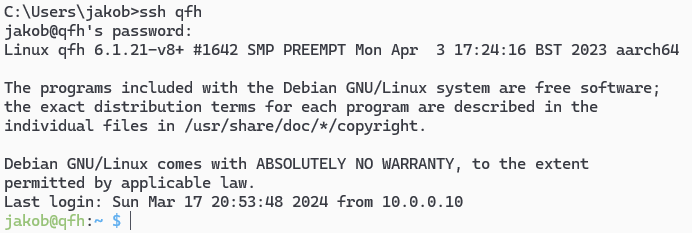
\includegraphics[width=\linewidth]{../ref/successfull_login.png}
	\caption{Erfolgreiche Verbindung über SSH}
	\label{fig:htrl-uhf(test)successfulllogin}
\end{figure}

\subsection{Hauptmenü}
Mithilfe des Befehls \textbf{sudo satnogs-setup} öffnet sich das Hauptmenü des SatNOGS Client über welches alle Einstellungen vorgenommen werden können.

\begin{figure} [H]
	\centering
	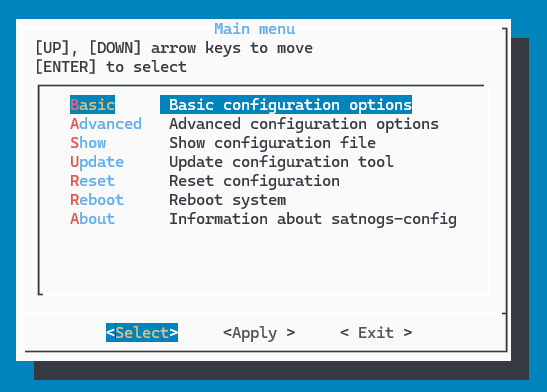
\includegraphics[width=.5\linewidth]{../ref/mainmenu.png}
	\caption{SatNOGS Client: Hauptmenü}
	\label{fig:mainmenu}
\end{figure}

Wurden alle Einstellungen vorgenommen so können diese mit \textbf{Apply} angewendet und gespeichert und angewendet werden.

\subsection{Einstellungen}
Wird im Hauptmenü der Reiter \textbf{Basic} mit \textbf{Enter} ausgewählt, so erscheint folgendes Fenster über welches alle grundlegenden Einstellungen zum Betrieb einer Empfangsstation vorgenommen werden können.

\begin{figure} [H]
	\centering
	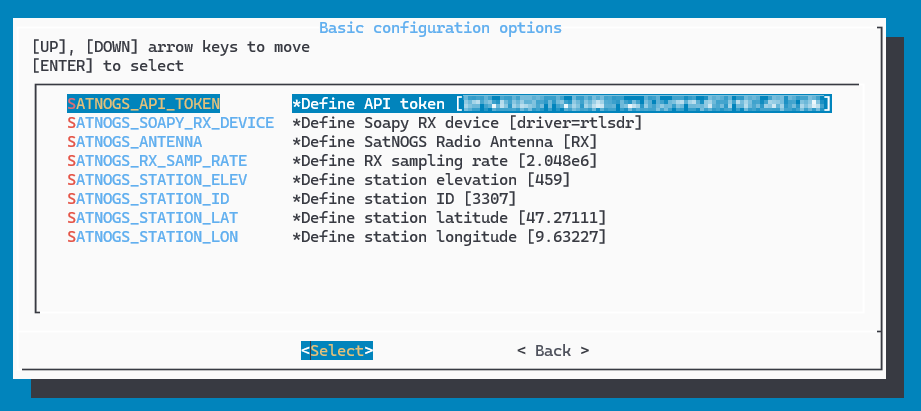
\includegraphics[width=.75\linewidth]{../ref/basic_configurations.png}
	\caption{SatNOGS Client: grundlegende Einstellungen}
	\label{fig:basic_configurations}
\end{figure}

\subsubsection{SATNOGS\textunderscore API\textunderscore TOKEN}
Der API-Schlüssel, welcher mit dem SatNOGS-Benutzerkonto verknüpft ist, wird von der Empfangsstation benötigt sich gegenüber der SatNOGS-Datenbank zu identifizieren und authentifizieren. Er kann auf dem Benutzerprofil der SatNOGS-Netzwerk Webseite durch das Klicken auf den in der folgenden Grafik mit 1 markierten Button an der mit 2 markierten Stelle abgelesen werden.

\begin{figure} [H]
	\centering
	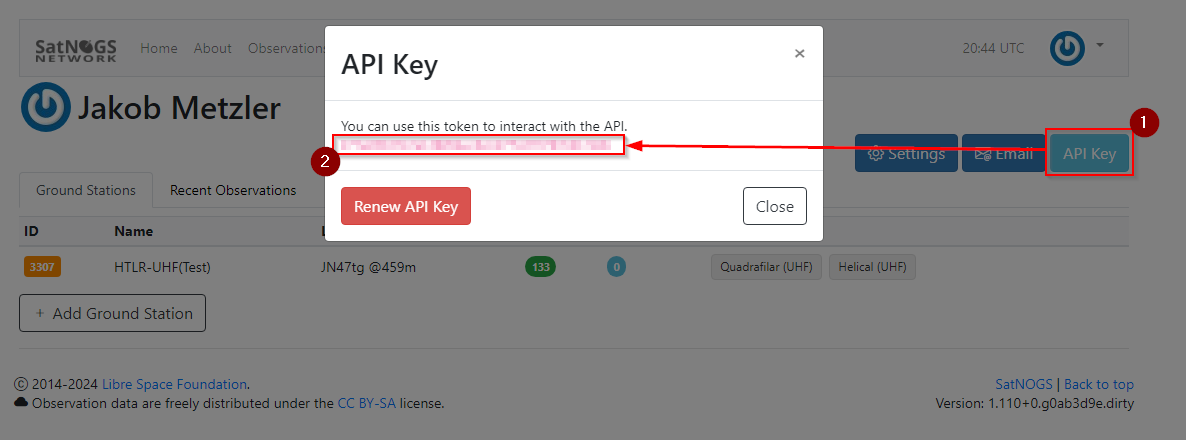
\includegraphics[width=.75\linewidth]{../ref/apitoken.png}
	\caption{SatNOGS-Netwerk Homepage: API-Schüssel ermitteln}
	\label{fig:apikey}
\end{figure}

\subsubsection{SATNOGS\textunderscore SOAPY\textunderscore RX\textunderscore DEVICE}
Mithilfe dieses Einstellungsparameters wird dem SatNOGS Client das verwendete SDR mitgeteilt. In diesem Fall entspricht das SDR dem, im späteren Kapitel \ref{sec:sdr} genauer Erläuterten, RTL-SDR Blog v3 und die dementsprechende einzugebende Treiber-Kennzeichnung lautet \textbf{driver=rtlsdr} \cite{noauthor_satnogsclient_nodate}. Weitere Treiber-Kennzeichnungen können auf der Software Defined Radio Seite des SatNOGS Wiki \cite{noauthor_software_nodate} nachgeschlagen werden.

\subsubsection{SATNOGS\textunderscore ANTENNA}
Über diesen Einstellungsparameter wird entsprechend dem verwendeten SDR und dem passenden Parameter der Modus des SDRs konfiguriert. Für das RTL-SDR Blog v3 entspricht das dem Parameter \textbf{RX} \cite{noauthor_satnogsclient_nodate}. Entsprechende Parameter für weitere SDR Typen können auf der Software Defined Radio Seite des SatNOGS Wiki \cite{noauthor_software_nodate} nachgeschlagen werden. 

\subsubsection{SATNOGS\textunderscore RX\textunderscore SAMP\textunderscore RATE}
Dieser Parameter legt die Abtastrate des SDRs fest. Für das RTL-SDR Blog v3 wird eine Abtastrate von 2.048 Megasamples pro Sekunde empfohlen \cite{noauthor_satnogsclient_nodate}, was über den Parameter 2.048e6 eingestellt werden kann. Auch hier finden sich für andere SDRs Informationen auf der Software Defined Radio Seite des SatNOGS Wiki \cite{noauthor_software_nodate}. 

\subsubsection{SATNOGS\textunderscore STATION\textunderscore ELEV}
Für diesen Parameter ist es notwendig die Höhenlage der Empfangsstation zu ermitteln. Es empfiehlt sich dazu eine interaktive topografische Karte, wie de-at.topographic-map.com, zu verwenden. Für den Standort der HTL Rankweil entspricht dieser Wert, was zugleich auch dem Parameter entspricht, 459 Meter. Dieser Wert wird für die Berechnungen der passierenden Satelliten und dessen Elevation- und Azimutalwinkel verwendet.

\subsubsection{SATNOGS\textunderscore STATION\textunderscore ID}
Die Station-ID wird zur eindeutigen Identifikation der Empfangsstation im SatNOGS-Netzwerk verwendet und kann auf der Seite des Benutzerprofils auf der Homepage des SatNOGS-Netzwerks abgelesen werden. 

\begin{figure} [H]
	\centering
	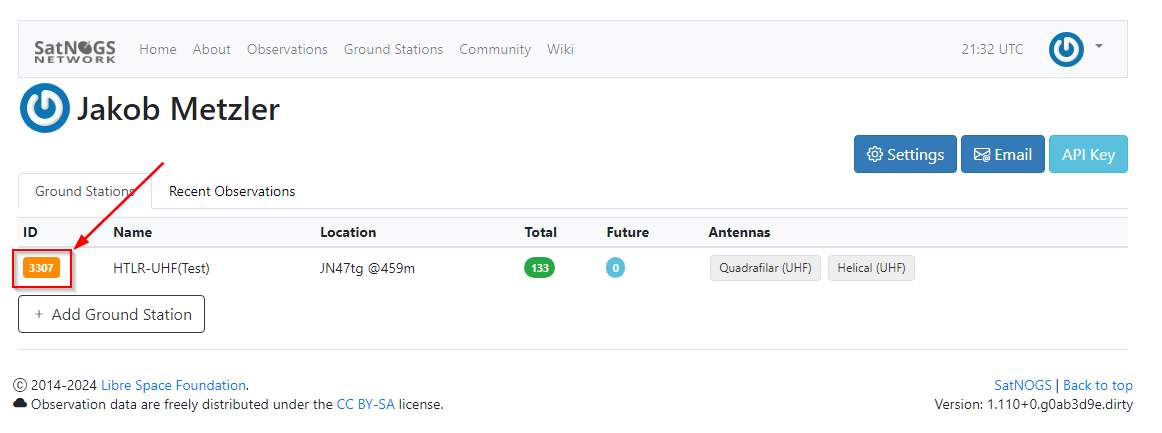
\includegraphics[width=.75\linewidth]{../ref/stationid.png}
	\caption{SatNOGS-Netzwerk Homepage: Station-ID ermitteln}
	\label{fig:stationid}
\end{figure}

\subsubsection{SATNOGS\textunderscore STATION\textunderscore LAT}
Dieser Parameter gibt den Breitengrad der Position der Empfangsstation an. Dieser Wert wird für die Berechnungen der passierenden Satelliten und dessen Elevation- und Azimutalwinkel verwendet.

\subsubsection{SATNOGS\textunderscore STATION\textunderscore LON}
Dieser Parameter gibt den Längengrad der Position der Empfangstation an. Dieser Wert wird für die Berechnungen der passierenden Satelliten und dessen Elevation- und Azimutalwinkel verwendet.

\section{erweiterte Konfiguration} 
Wird im Hauptmenü der Reiter \textbf{Advanced} mit \textbf{Enter} ausgewählt, so erscheint folgendes Fenster über welches erweiterte Einstellungen vorgenommen werden können. 

\begin{figure} [H]
	\centering
	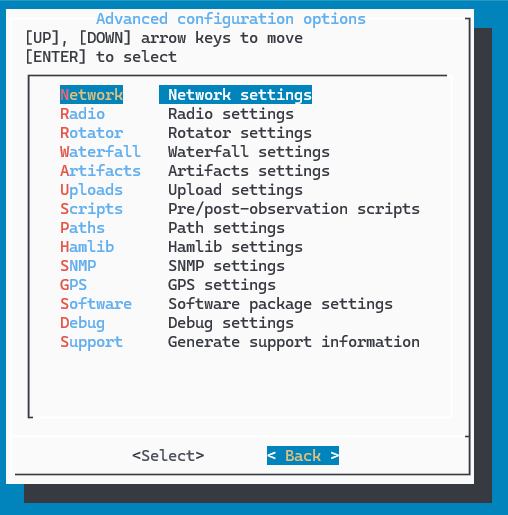
\includegraphics[width=.5\linewidth]{../ref/advanced_settings.png}
	\caption{SatNOGS Client: erweiterte Einstellungen}
	\label{fig:advanced_settings}
\end{figure}

Die wichtigsten Einstellungen die hier vorgenommen werden können sind das definieren der Verstärkung des SDRs, das Einrichten einer Unterstützung für die Verwendung eines Rotors und das automatische Aktivieren von Bias-T während einer Observation.

\subsection{Verstärkung des SDRs einstellen}
Um die Verstärkung des SDRs einzustellen müssen zuerst die möglichen Parameter ermittelt werden, was durch das ausführen des Befehls \textbf{rtl\textunderscore test} in der SSH gemacht werden kann. 

\begin{figure} [H]
	\centering
	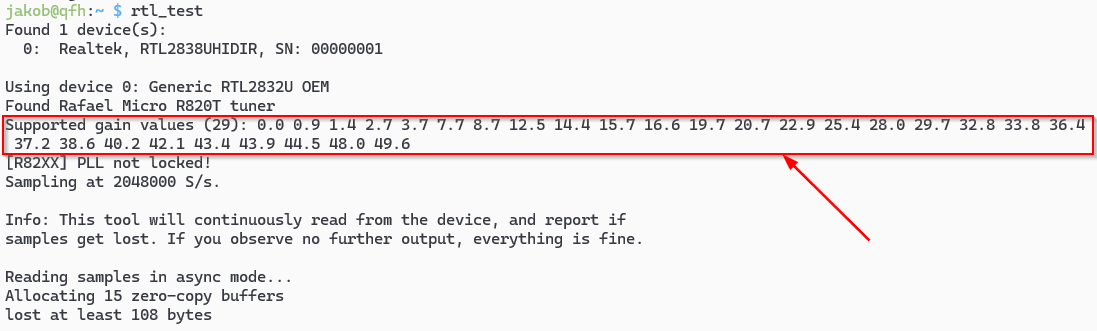
\includegraphics[width=\linewidth]{../ref/supportedgain.png}
	\caption{SatNOGS Client: unterstützte Gain Werte ermitteln}
	\label{fig:supportedgain}
\end{figure}

Wurde aus der Ausgabe, wie in obiger Darstellung gezeigt, der gewünschte Wert der Verstärkung gewählt, so kann dieser in den erweiterten Einstellungen unter dem Reiter \textbf{Radio} mithilfe des Parameters \textbf{SATNOGS\textunderscore RF\textunderscore GAIN} eingestellt werden. 

\subsection{Rotor-Unterstützung implementieren}
Für die Implementierung einer Rotorsteuerung müssen in den erweiterten Einstellungen unter dem Reiter \textbf{Rotator} drei Parameter angepasst werden. 

Der erste Parameter \textbf{SATNOGS\textunderscore ROT\textunderscore ENABLED} aktiviert die Verwendung der konfigurierten Rotorsteuerung. 

Mithilfe des Parameters \textbf{SATNOGS\textunderscore ROT\textunderscore MODEL} wird das Model der Rotorsteuerung festgelegt. Im Fall der im späteren Kapitel \ref{sec:gs232emulation} erläuterten GS232A/B Steuerung wird für den Parameter \textbf{ROT\textunderscore MODEL\textunderscore GS232B} verwendet \cite{noauthor_satnogsclient_nodate}. 

\textbf{SATNOGS\textunderscore ROT\textunderscore BAUD} legt die Baud-Rate der Kommunikation mit der Steuerung fest und beträgt im Fall der im späteren Kapitel \ref{sec:gs232emulation} erläuterten Steuerung 9600.

\subsection{Aktivieren von Bias-T}
Das Aktivieren von Bias-T ist abhängig vom verwendeten SDR und wird nun nur für das RTL-SDR Blog v3 erläutert. Um die softwaremäßigen Voraussetzungen für die Verwendung von Bias-T am RTL-SDR Blog v3 zu erfüllen müssen im ersten Schritt folgende Befehle in der SSH ausgeführt werden:
\newline 1. \textbf{sudo apt install cmake}
\newline 2. \textbf{git clone https://github.com/rtlsdrblog/rtl\textunderscore biast}
\newline 3. \textbf{cd rtl\textunderscore biast}
\newline 4. \textbf{mkdir build}
\newline 5. \textbf{cd build}
\newline 6. \textbf{cmake ..}
\newline 7. \textbf{make}

Diese Schritte ermöglichen die Kontrolle der Bias-T Funktion des RTL-SDR Blog v3 und müssen nur einmal durchgeführt werden. Sie ermöglichen die Kontrolle der Funktion über folgende Befehle:
\newline Einschalten: \textbf{/rtl\textunderscore biast/build/src/rtl\textunderscore biast -b 1}
\newline Ausschalten: \textbf{/rtl\textunderscore biast/build/src/rtl\textunderscore biast -b 0}

Diese Befehle können nun in den erweiterten Einstellungen unter dem Reiter Scripts als Pre- und Post-Observation Script festgelegt werden. Dazu wird der Einschalt- sowie Ausschaltbefehl mit \textbf{/home} am Anfang, aufgrund des Ursprungsverzeichnisses des SatNOGS Client, erweitert werden.		% INCLUDE Groundstation setup
\chapter{Simulation}
\label{chap:sim}

\section{Quadrifilare Helix-Antenne (QFH)}
\label{sec:QFH}

\subsection{3D-Modelle}
\label{subsec:3D-mod-qfh}

\subsection{CENOS}
\label{subsec:cenos-qfh}

\section{gerichtete Helix-Antenne}
\label{sec:Helix}

\subsection{3D-Modelle}
\label{subsec:3D-mod-helix}

\subsection{CENOS}
\label{subsec:cenos-helix}	% INCLUDE Simulation results
\chapter{Konstruktion der Antennen}
\label{chap:cons}

\section{Quadrifilare Helix-Antenne (QFH)}
\label{cons-qfh}

\section{gerichtete Helix-Antenne}
\label{cons-helix} % INCLUDE Construction info
\chapter{Discussion}
\label{chap:disc}
\vspace*{3cm}
\section{Summary of findings}
\Blindtext[1]
\vfill   % INCLUDE Discussion
\chapter{Conclusio}

Mit dem Abschluss der Diplomarbeit wurden die gesteckten Ziele erfolgreich erreicht und wichtige Erkenntnisse gewonnen. Die Arbeit präsentiert ein funktionierendes Konzept für den Bau einer Empfangsstation im globalen Satellitenkommunikationsnetzwerk SatNOGS, das die flächenmäßige Abdeckung erweitert und die Ausfallsicherheit erhöht.

Die Erfahrungen aus dem Bau der quadrifilaren Helixantenne erwiesen sich als äußerst wertvoll beim Bau der monofilaren Helixantenne, was zu einem ausgereiften Antennenarray führte. Unter Berücksichtigung des finanziellen Aspekts ist festzustellen, dass selbst bei geringerem finanziellen Aufwand, wie es bei einer quadrifilaren Helixantenne der Fall ist, eine zuverlässige Antenne und somit eine erschwingliche Empfangsstation für den Empfang von Daten wissenschaftlicher Satelliten realisiert werden kann.

In Anbetracht der Kosteneffizienz der quadrifilaren Helixantenne ist es sinnvoll, ihre Entwicklung fortzusetzen. Dies könnte durch eine eingehende Untersuchung und Analyse der Abweichungen zwischen der gemessenen Richtwirkung und den Simulationsergebnissen erfolgen, sowie durch die Prüfung der Auswirkungen der Form des Materials zur Modellierung der Schleifen auf die Antenneneigenschaften.

Die im Pflichtenheft festgelegte Dekodierung und Darstellung der empfangenen Daten für den CubeSat des TU Wien Space Team konnte nicht durchgeführt werden, da das dafür benötigte Protokoll noch nicht vollständig vom Space Team entwickelt wurde.   % INCLUDE Conclusion
\chapter{Perspektiven}
\label{chap:persp}
konischer Reflektor...
 % INCLUDE Perspectives


% -------------------------- 
% Back matter
% --------------------------
\chapter{Literaturverzeichnis}
\vspace{1cm}
\printbibliography[heading=none]

% ********************************************************* 
% END OF THESIS
% *********************************************************
\end{document}